\documentclass[aspectratio=1610,onlymath]{beamer}
% \documentclass[aspectratio=1610,onlymath,handout]{beamer}

\input{macros-lecture}
% Common notation

\usepackage{amsmath,amssymb,amsfonts}
\usepackage{xspace}

\newcommand{\lectureurl}{https://iccl.inf.tu-dresden.de/web/FS2023}

\DeclareMathAlphabet{\mathsc}{OT1}{cmr}{m}{sc} % Let's have \mathsc since the slide style has no working \textsc

% Dual of "phantom": make a text that is visible but intangible
\newcommand{\ghost}[1]{\raisebox{0pt}[0pt][0pt]{\makebox[0pt][l]{#1}}}

\newcommand{\tuple}[1]{\langle{#1}\rangle}
\newcommand{\defeq}{\mathrel{:=}}

%%% Annotation %%%

\usepackage{color}
\newcommand{\todo}[1]{{\tiny\color{red}\textbf{TODO: #1}}}



%%% Old macros below; move when needed

\newcommand{\blank}{\text{\textvisiblespace}} % empty tape cell for TM

% table syntax
\newcommand{\dom}{\textbf{dom}}
\newcommand{\adom}{\textbf{adom}}
\newcommand{\dbconst}[1]{\texttt{"#1"}}
\newcommand{\pred}[1]{\textsf{#1}}
\newcommand{\foquery}[2]{#2[#1]}
\newcommand{\ground}[1]{\textsf{ground}(#1)}
% \newcommand{\foquery}[2]{\{#1\mid #2\}} %% Notation as used in Alice Book
% \newcommand{\foquery}[2]{\tuple{#1\mid #2}}

\newcommand{\quantor}{\mathord{\reflectbox{$\text{\sf{Q}}$}}} % the generic quantor

% logic syntax
\newcommand{\Inter}{\mathcal{I}} %used to denote an interpretation
\newcommand{\Jnter}{\mathcal{J}} %used to denote another interpretation
\newcommand{\Knter}{\mathcal{K}} %used to denote yet another interpretation
\newcommand{\Zuweisung}{\mathcal{Z}} %used to denote a variable assignment

% query languages
\newcommand{\qlang}[1]{{\sf #1}} % Font for query languages
\newcommand{\qmaps}[1]{\textbf{QM}({\sf #1})} % Set of query mappings for a query language

%%% Complexities %%%

\hyphenation{Exp-Time} % prevent "Ex-PTime" (see, e.g. Tobies'01, Glimm'07 ;-)
\hyphenation{NExp-Time} % better that than something else

% \newcommand{\complclass}[1]{{\sc #1}\xspace} % font for complexity classes
\newcommand{\complclass}[1]{\ensuremath{\mathsc{#1}}\xspace} % font for complexity classes

\newcommand{\ACzero}{\complclass{AC$_0$}}
\newcommand{\LogSpace}{\complclass{L}}
\newcommand{\NLogSpace}{\complclass{NL}}
\newcommand{\PTime}{\complclass{P}}
\newcommand{\NP}{\complclass{NP}}
\newcommand{\coNP}{\complclass{coNP}}
\newcommand{\PH}{\complclass{PH}}
\newcommand{\PSpace}{\complclass{PSpace}}
\newcommand{\NPSpace}{\complclass{NPSpace}}
\newcommand{\ExpTime}{\complclass{ExpTime}}
\newcommand{\NExpTime}{\complclass{NExpTime}}
\newcommand{\ExpSpace}{\complclass{ExpSpace}}
\newcommand{\TwoExpTime}{\complclass{2ExpTime}}
\newcommand{\NTwoExpTime}{\complclass{N2ExpTime}}
\newcommand{\ThreeExpTime}{\complclass{3ExpTime}}
\newcommand{\kExpTime}[1]{\complclass{#1ExpTime}}
\newcommand{\kExpSpace}[1]{\complclass{#1ExpSpace}}


\defineTitle{9}{Minimale Automaten (2)}{23. November 2020}

\begin{document}

\maketitle

\sectionSlideNoHandout{Rückblick}

\begin{frame}\frametitle{Automaten verkleinern mit Quotientenbildung}

Wir betrachten DFAs mit totaler Übergangsfunktion.\medskip

{\begin{tikzpicture}[baseline={(current bounding box.center)}]
\draw[dashed,fill=strongyellow!30] (-0.8,-0.9) rectangle node[above,yshift=-1.50cm,xshift=-0.0cm] {\footnotesize$[A]_\sim = [C]_\sim =\{A,C\}$}(2.0,2.0);
\draw[dashed,fill=strongyellow!30] (2.2,-0.9) rectangle node[above,yshift=-1cm,xshift=-0.0cm] {\footnotesize$[B]_\sim =\{B\}$}(3.6,1.0);
% \draw[help lines] (0,0) grid (7,2);
\node (s1) [circle,draw=black,thick] at (0,0) {$A$};
\node (s2) [circle,draw=black,thick,double] at (3,0) {$B$};
\node (s3) [circle,draw=black,thick] at (1.5,1.5) {$C$};
%
\path[->,line width=0.5mm](-1,0) edge (s1);
\path[->,line width=0.5mm](s1) edge node[below] {\Sterm{0}} (s2);
\path[->,line width=0.5mm](s1) edge node[left] {\Sterm{1}} (s3);
\path[->,line width=0.5mm](s3) edge node[right] {\Sterm{0}} (s2);
\path[->,line width=0.5mm](s3) edge [loop above] node[above] {\Sterm{1}} (s3);
\end{tikzpicture}\hspace{3cm}
%
\begin{minipage}{3.5cm}
Ermittlung der\\ Zustandsäquivalenz $\sim$:

\begin{tabular}{c|c|c|}
 \multicolumn{1}{c}{}  & \multicolumn{1}{c}{A} & \multicolumn{1}{c}{B} \\\cline{2-3}
 C &   &   $\epsilon$ \\\cline{2-3}
 B & $\epsilon$ \\\cline{2-2}
\end{tabular}
\end{minipage}}
\bigskip

 
\begin{minipage}{5.5cm}
{Quotientenautomat:\\[1ex]
%
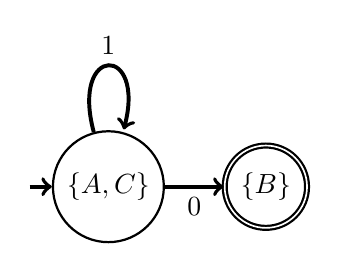
\begin{tikzpicture}[baseline={(current bounding box.center)}]
% \draw[help lines] (0,0) grid (7,2);
\node (s1) [circle,draw=black,thick] at (0,0) {$\{A,C\}$};
\node (s2) [circle,draw=black,thick,double] at (2,0) {$\{B\}$};
%
\path[->,line width=0.5mm](-1,0) edge (s1);
\path[->,line width=0.5mm](s1) edge node[below] {\Sterm{0}} (s2);
\path[->,line width=0.5mm](s1) edge [loop above] node[above] {\Sterm{1}} (s1);
\end{tikzpicture}}
\end{minipage}
\begin{minipage}{6cm}\footnotesize
\defbox{Sei $\Smach{M}$ ein DFA mit totaler Übergangsfunktion.
Der \redalert{reduzierte Automat $\Smach{M}_r$} ergibt sich durch folgende Schritte:
\begin{enumerate}[(1)]
\item Entferne alle unerreichbaren Zustände aus $\Smach{M}$
\item Berechne den Quotientenautomaten
\end{enumerate}
}
\end{minipage}

\end{frame}


\begin{frame}[t]\frametitle{Verschiedene Äquivalenzrelationen}

Für einen DFA $\Smach{M}$ und eine Sprache $\Slang{L}$ haben wir verschiedene
Äquivalenzrelationen verwendet:
\medskip

\defbox{\redalert{DFA-Zustandsäquivalenz} ${\sim_{\Smach{M}}}\subseteq Q\times Q$:\\ $q\sim_{\Smach{M}}p$ wenn
für alle $w\in\Sigma^*$ gilt: $\delta(q,w)\in F$ gdw. $\delta(p,w)\in F$.}%
\medskip

\alert{Anwendung:} Vereinfachung von DFAs durch Quotientenbildung
\medskip

\defbox{\redalert{Nerode-Rechtskongruenz} ${\simeq_{\Slang{L}}}\subseteq \Sigma^*\times \Sigma^*$:\\ $u\simeq_{\Slang{L}}v$ wenn
für alle $w\in\Sigma^*$ gilt: $uw\in\Slang{L}$ gdw. $vw\in\Slang{L}$.}%
\medskip

\alert{Anwendung:} automatenunabhängige Analyse von Sprachen; alternative Konstruktion Minimalautomat
\medskip

% \defbox{\redalert{DFA-Präfixäquivalenz} ${\simeq_{\Smach{M}}}\subseteq \Sigma^*\times \Sigma^*$:\\ $u\simeq_{\Smach{M}}v$ wenn
% gilt: $\delta(q_0,u)=\delta(q_0,v)$.}%
% \medskip
% 
% \alert{Anwendung:} Beweis des Satzes von Myhill \& Nerode


\end{frame}

\sectionSlide{Der Satz von Myhill und Nerode}


\begin{frame}[t]\frametitle{$\simeq$ und reguläre Sprachen}

\theobox{\emph{Satz:} Wenn $\Slang{L}$ regulär ist, dann hat $\simeq_{\Slang{L}}$ endlich viele Äquivalenzklassen.}
(Die Zahl der Äquivalenzklassen wird auch als \redalert{Index} bezeichnet)\medskip\pause

\emph{Beweis:} Wir erhalten diese Eigenschaft aus der Darstellung von $\Slang{L}$ mit einem DFA.

\defbox{Für einen DFA $\Smach{M}=\tuple{Q,\Sigma,\delta,q_0,F}$ definieren wir eine Relation $\simeq_{\Smach{M}}$ wie folgt.
Für Wörter $u,v\in\Sigma^*$ sei $u\simeq_{\Smach{M}}v$ wenn gilt:\\[1ex]
\narrowcentering{$\delta(q_0,u)=\delta(q_0,v)$.}
}

Offensichtlich ist $\simeq_{\Smach{M}}$ eine Äquivalenzrelation (Eigenschaften "`geerbt"' von $=$) mit endlichem Index (es gibt nur endlich viele Zustände).
\medskip

% Wir beweisen die Behauptung, indem wir zeigen:\\
% wenn $u \simeq_{\Smach{M}} v$ dann $u \simeq_{\Slang{L}} v$, d.h. ${\simeq_{\Smach{M}}}\subseteq {\simeq_{\Slang{L}}}$.
% \\
% (denn dann hat $\simeq_{\Slang{L}}$ )

\end{frame}

\begin{frame}[t]\frametitle{$\simeq$ und reguläre Sprachen (2)}

\theobox{\emph{Satz:} Wenn $\Slang{L}$ regulär ist, dann hat $\simeq_{\Slang{L}}$ endlich viele Äquivalenzklassen.}

\emph{Beweis (Fortsetzung):} 
Behauptung: ${\simeq_{\Smach{M}}}\subseteq {\simeq_{\Slang{L}}}$ das heißt\\[1ex]
% 
\narrowcentering{wenn $u \simeq_{\Smach{M}} v$ dann $u \simeq_{\Slang{L}} v$}.\medskip

Wir betrachten einen DFA $\Smach{M}$ mit $\Slang{L}=\Slang{L}(\Smach{M})$.\pause
\begin{itemize}
\item Seien $u,v\in\Sigma^*$ Wörter mit $u \simeq_{\Smach{M}} v$\pause
\item Dann ist $\delta(q_0,u)=\delta(q_0,v)$\pause
\item Dann gilt, für alle $w\in\Sigma^*$, $\delta(q_0,uw)=\delta(q_0,vw)$\pause
\item Dann gilt, für alle $w\in\Sigma^*$, $\delta(q_0,uw)\in F$ gdw. $\delta(q_0,vw)\in F$\pause
\item Dann gilt, für alle $w\in\Sigma^*$, $uw\in \Slang{L}(\Smach{M})$ gdw. $vw\in \Slang{L}(\Smach{M})$\pause
\item Dann ist $u \simeq_{\Slang{L}(\Smach{M})} v$ und also $u \simeq_{\Slang{L}} v$
\end{itemize}
Damit ist die Behauptung gezeigt.

\end{frame}

\begin{frame}[t]\frametitle{$\simeq$ und reguläre Sprachen (3)}

\theobox{\emph{Satz:} Wenn $\Slang{L}$ regulär ist, dann hat $\simeq_{\Slang{L}}$ endlich viele Äquivalenzklassen.}

\emph{Beweis (Fortsetzung):} Wir haben gezeigt, dass ${\simeq_{\Smach{M}}}\subseteq {\simeq_{\Slang{L}}}$.\pause
\medskip

\begin{enumerate}[$\leadsto$]
\item Jede ${\simeq_{\Slang{L}}}$-Äquivalenzklasse besteht aus einer oder mehr ${\simeq_{\Smach{M}}}$-Äquivalenzklassen\pause
\item Der Index von ${\simeq_{\Slang{L}}}$ ist kleiner oder gleich dem Index von ${\simeq_{\Smach{M}}}$\pause
\item Der Index von ${\simeq_{\Slang{L}}}$ ist endlich \qed
\end{enumerate}
\medskip

\textcolor{devilscss}{\footnotesize Anmerkung: Der letzte Teil ist eine allgemeine Eigenschaft aller Äquivalenzrelationen: wenn $R\subseteq S$, dann ist der Index von $R$ größer oder gleich dem Index von $S$.}

\end{frame}

\begin{frame}[t]\frametitle{Verschiedene Äquivalenzrelationen}

Für einen DFA $\Smach{M}$ und eine Sprache $\Slang{L}$ haben wir verschiedene
Äquivalenzrelationen verwendet:
\medskip

\defbox{\redalert{DFA-Zustandsäquivalenz} ${\sim_{\Smach{M}}}\subseteq Q\times Q$:\\ $q\sim_{\Smach{M}}p$ wenn
für alle $w\in\Sigma^*$ gilt: $\delta(q,w)\in F$ gdw. $\delta(p,w)\in F$.}%
\medskip

\alert{Anwendung:} Vereinfachung von DFAs durch Quotientenbildung
\medskip

\defbox{\redalert{Nerode-Rechtskongruenz} ${\simeq_{\Slang{L}}}\subseteq \Sigma^*\times \Sigma^*$:\\ $u\simeq_{\Slang{L}}v$ wenn
für alle $w\in\Sigma^*$ gilt: $uw\in\Slang{L}$ gdw. $vw\in\Slang{L}$.}%
\medskip

\alert{Anwendung:} automatenunabhängige Analyse von Sprachen; alternative Konstruktion Minimalautomat
\medskip

\defbox{\redalert{DFA-Präfixäquivalenz} ${\simeq_{\Smach{M}}}\subseteq \Sigma^*\times \Sigma^*$:\\ $u\simeq_{\Smach{M}}v$ wenn
gilt: $\delta(q_0,u)=\delta(q_0,v)$.}%
\medskip

\alert{Anwendung:} Beweis der Endlichkeit des $\simeq_{\Slang{L}}$-Indexes regulärer Sprachen


\end{frame}


\begin{frame}\frametitle{Der Satz von Myhill und Nerode}

Das vorige Resultat kann noch verstärkt werden:

\theobox{\emph{Satz (Myhill \& Nerode):} Eine Sprache $\Slang{L}$ ist genau dann regulär, wenn $\simeq_{\Slang{L}}$ endlich viele Äquivalenzklassen hat.}\pause

\emph{Beweis:}
Die Richtung "`$\Rightarrow$"' haben wir soeben gezeigt.\pause\medskip

Für die Richtung "`$\Leftarrow$"' zeigen wir, wie man einen DFA $\Smach{M}_{\Slang{L}}$ für $\Slang{L}$ erhalten kann, wenn $\simeq_{\Slang{L}}$ endlich viele Äquivalenzklassen hat.\pause

\codebox{Der DFA $\Smach{M}_{\Slang{L}}=\tuple{Q,\Sigma,\delta,q_0,F}$ ist wie folgt definiert:
\begin{itemize}
\item $Q=\{[w]_\simeq\mid w\in\Sigma^*\}$ ist die (endliche) Menge der $\simeq$-Äquivalenzklassen
\item $q_0=[\epsilon]_\simeq$
\item $F=\{[w]_\simeq\mid w\in\Slang{L}\}$
\item $\delta([w]_\simeq,\Sterm{a})=[w\Sterm{a}]_\simeq$
\end{itemize}
}\vspace{-1ex}
{\tiny Anmerkung: Diese Definition von $F$ und $\delta$ ist zulässig, weil sie nicht vom gewählten Repräsentanten $w$ abhängt}\\[-1.5ex]{\tiny (da $\simeq$ eine Rechtskongruenz ist)}

\end{frame}


\begin{frame}\frametitle{Satz von Myhill und Nerode: Beweis}

\emph{Beweis (Fortsetzung):} Wir müssen noch zeigen, dass $\Slang{L}=\Slang{L}(\Smach{M}_{\Slang{L}})$.
%
\[\begin{array}{r@{~\text{ gdw. }~}ll}
w\in\Slang{L}(\Smach{M}_{\Slang{L}}) & \delta(q_0,w)\in F \\\pause
	& \delta([\epsilon]_\simeq,w)\in F \\\pause
	& [w]_\simeq\in F & \text{wegen $\delta([u],v)=[uv]$ }\\
	\multicolumn{2}{c}{} & \text{(Induktion über $|v|$) }\\\pause
	& w\in \Slang{L}
\end{array}
\]
\qed

\end{frame}

\begin{frame}\frametitle{Beispiel}

Die Konstruktion von Myhill \& Nerode für die Sprache
$\Slang{L}= \{ w\mid w\text{ enthält kein Infix }\Sterm{ab} \}$ über dem Alphabet $\Sigma=\{\Sterm{a},\Sterm{b},\Sterm{c}\}$
\medskip

\begin{tabular}{lll}
 & erlaubte Suffixe $w$ & \\[-1ex]
Klasse $C$ & mit $C\cdot\{w\}\subseteq\Slang{L}$ & $C$ als Menge\\\hline
\pause $[\epsilon]_\simeq$ & \pause $w\in\Slang{L}$ & \pause$\{ v\in\Slang{L}\mid v\text{ endet nicht auf }\Sterm{a} \}$ \\\pause
$[\Sterm{a}]_\simeq$ & \pause$w\in\Slang{L}$, $w$ beginnt nicht mit $\Sterm{b}$ & \pause$\{ v\in\Slang{L}\mid v\text{ endet auf }\Sterm{a} \}$ \\\pause
$[\Sterm{ab}]_\simeq$ & \pause keine & \pause$\{ v\mid v\notin\Slang{L} \}$\pause
\end{tabular}

\bigskip
\narrowcentering{%
\begin{tikzpicture}[baseline={(current bounding box.center)}]
% \draw[help lines] (0,0) grid (7,2);
\node (s1) [circle,draw=black,thick,onslide={<12->{double}}] at (0,0) {$[\epsilon]_\simeq$};
\node (s2) [circle,draw=black,thick,onslide={<12->{double}}] at (2,0) {$[\Sterm{a}]_\simeq$};
\node (s3) [circle,draw=black,thick] at (4,0) {$[\Sterm{ab}]_\simeq$};
%
\path[->,line width=0.5mm](-1,0) edge (s1);
\onslide<13->{\path[->,line width=0.5mm,bend left](s1) edge node[above] {\Sterm{a}} (s2);}
\onslide<14->{\path[->,line width=0.5mm](s2) edge node[above] {\Sterm{b}} (s3);}
\onslide<17->{\path[->,line width=0.5mm](s1) edge [loop above] node[above] {\Sterm{b},\Sterm{c}} (s1);}
\onslide<15->{\path[->,line width=0.5mm](s2) edge [loop above] node[above] {\Sterm{a}} (s2);}
\onslide<16->{\path[->,line width=0.5mm,bend left](s2) edge node[below] {\Sterm{c}} (s1);}
\onslide<18->{\path[->,line width=0.5mm](s3) edge [loop above] node[above] {\Sterm{a},\Sterm{b},\Sterm{c}} (s3);}
\end{tikzpicture}}

\end{frame}


\begin{frame}[t]\frametitle{$\Smach{M}_{\Slang{L}}$ ist minimal}

Für reguläre $\Slang{L}$ haben wir bereits gezeigt:
\theobox{\vspace{-1ex}
\begin{itemize}
\item $\Smach{M}_{\Slang{L}}$ ist ein DFA, da er insbesondere endlich viele Zustände hat (Index von $\simeq$)
\item $\Slang{L}(\Smach{M}_{\Slang{L}})=\Slang{L}$
\end{itemize}}%
\medskip

Als nächstes interessiert uns der Bezug zum Minimalautomat\pause:

\theobox{\emph{Satz:} $\Smach{M}_{\Slang{L}}$ hat unter allen totalen DFAs, die $\Slang{L}$ erkennen, eine minimale Anzahl an Zuständen.}\pause

\emph{Beweis:} Sei $\Smach{M}$ ein beliebiger totaler DFA mit $\Slang{L}(\Smach{M})=\Slang{L}$
\begin{itemize}
\item Wir haben bereits gezeigt: ${\simeq_{\Smach{M}}}\subseteq{\simeq_{\Slang{L}}}$
\item Daraus folgerten wir:\\ "`Zahl der $\simeq_{\Slang{L}}$-Äquivalenzklassen $\leq$ Anzahl der erreichbaren Zustände von $\Smach{M}$"'
\item Die Zahl der $\simeq_{\Slang{L}}$-Äquivalenzklassen ist aber die Anzahl der Zustände von $\Smach{M}_{\Slang{L}}$\qed
\end{itemize}

\end{frame}

\begin{frame}[t]\frametitle{Weitere Eigenschaften von $\Smach{M}_{\Slang{L}}$}

Für reguläre $\Slang{L}$ haben wir bereits gezeigt:
\theobox{\vspace{-1ex}
\begin{itemize}
\item $\Smach{M}_{\Slang{L}}$ ist ein DFA, da er insbesondere endlich viele Zustände hat (Index von $\simeq$)
\item $\Slang{L}(\Smach{M}_{\Slang{L}})=\Slang{L}$
\item Jeder Zustand von $\Smach{M}_{\Slang{L}}$ ist vom Startzustand aus erreichbar, da $\delta([\epsilon]_\simeq,w)=[w]_\simeq$
\item ${\simeq_{\Smach{M}_{\Slang{L}}}}={\simeq_{\Slang{L}}}$ \only<2->{($\spadesuit$)}
\end{itemize}}%
\medskip\pause

\emph{Beweis ($\spadesuit$):} ${\simeq_{\Smach{M}_{\Slang{L}}}}\subseteq{\simeq_{\Slang{L}}}$ haben wir bereits für beliebige DFA gezeigt
\medskip

${\simeq_{\Smach{M}_{\Slang{L}}}}\supseteq{\simeq_{\Slang{L}}}$ kann wie folgt gezeigt werden:
\begin{itemize}
\item Seien $u,v\in\Sigma^*$ beliebige Wörter mit $u\simeq_{\Slang{L}} v$
\item Dann gilt für $\Smach{M}_{\Slang{L}}$: $\delta([\epsilon]_\simeq,u)=[u]_\simeq=[v]_\simeq=\delta([\epsilon]_\simeq,v)$
\item Also ist $u\simeq_{\Smach{M}_{\Slang{L}}} v$\qed
\end{itemize}

\end{frame}

\begin{frame}\frametitle{Isomorphismen von Automaten}

"`Isomorph"' bedeutet "`gleich bis auf Umbenennung von Zuständen"':\bigskip

\defbox{Ein \redalert{Isomorphismus} zwischen zwei DFAs $\Smach{M}_1=\tuple{Q_1,\Sigma,\delta_1,q_1,F_1}$ und $\Smach{M}_2=\tuple{Q_2,\Sigma,\delta_2,q_2,F_2}$
ist eine bijekive Funktion $f:Q_1\to Q_2$, so dass gilt:
\begin{itemize}
\item $f(q_1)=q_2$
\item $f(\delta_1(q,\Sterm{a})) = \delta_2(f(q),\Sterm{a})$ für alle $\Sterm{a}\in\Sigma$
\item $\{f(q)\mid q\in F_1\}=F_2$
\end{itemize}
Zwei Automaten sind \redalert{isomorph}, wenn es einen Isomorphismus zwischen ihnen gibt.
}%
\bigskip

Man kann leicht zeigen, dass isomorphe Automaten die selbe Sprache akzeptieren
\bigskip

% Wir wollen zeigen: jeder reduzierte der Myhill-Nerode-Minimalautomat

\end{frame}


\begin{frame}[t]\frametitle{Eindeutigkeit des Minimalautomaten}

\theobox{\emph{Satz:} Ist $\Slang{L}$ eine reguläre Sprache, $\Smach{M}$ ein DFA mit totaler Übergangsfunktion
und $\Slang{L}(\Smach{M})=\Slang{L}$, so sind der reduzierte Automat $\Smach{M}_r$ und der Myhill-Nerode-Minimalautomat $\Smach{M}_{\Slang{L}}$ isomorph.}

\emph{Beweis:}
Sei $\Smach{M}_{\Slang{L}}=\tuple{Q,\Sigma,\delta,q,F}$ und $\Smach{M}_r=\tuple{Q_r,\Sigma,\delta_r,q_r,F_r}$.
\medskip

\begin{minipage}{4cm}
\codebox{$\Smach{M}_{\Slang{L}}=\tuple{Q,\Sigma,\delta,q_0,F}$ mit:
\begin{itemize}
\item $Q=\{[w]_\simeq\mid w\in\Sigma^*\}$
\item $q_0=[\epsilon]_\simeq$
\item $F=\{[w]_\simeq\mid w\in\Slang{L}\}$
\item $\delta([w]_\simeq,\Sterm{a})=[w\Sterm{a}]_\simeq$
\end{itemize}
}
\end{minipage}\hspace{1cm}
\begin{minipage}{4.5cm}\codebox{$\Smach{M}_r=\tuple{Q_r,\Sigma,\delta_r,q_r,F_r}$:
\begin{enumerate}[(1)]
\item Entferne unerreichbare Zustände
\item Berechne den Quotienten-DFA bzgl. $\sim$
\end{enumerate}}
\end{minipage}\pause\bigskip

Wir definieren eine Funktion $f: Q_r\to Q$ wie folgt:\\[1ex]

\codebox{%
\narrowcentering{für $q\in Q_r$ wähle ein Wort $w$ mit $\delta_r(q_r,w)=q$ und setze $f(q)=[w]_\simeq$}}
% 
% \begin{itemize}
% \item für jeden Zustand $q\in Q_r$ gibt es ein Wort $w$ mit $\delta(q_0,w)=q$\\[-0.7ex] {\tiny (Erreichbarkeit aller Zustände)}
% \item wir definieren $f(q)=[w]_\simeq$ für ein solches Wort $w$
% \end{itemize}

\end{frame}

\begin{frame}[t]\frametitle{Eindeutigkeit des Minimalautomaten (2)}

% \begin{minipage}{4cm}
% \codebox{$\Smach{M}_{\Slang{L}}=\tuple{Q,\Sigma,\delta,q_0,F}$ mit:
% \begin{itemize}
% \item $Q=\{[w]_\simeq\mid w\in\Sigma^*\}$
% \item $q_0=[\epsilon]_\simeq$
% \item $F=\{[w]_\simeq\mid w\in\Slang{L}\}$
% \item $\delta([w]_\simeq,\Sterm{a})=[w\Sterm{a}]_\simeq$
% \end{itemize}
% }
% \end{minipage}\hspace{1cm}
% \begin{minipage}{4.5cm}\codebox{$\Smach{M}_r=\tuple{Q_r,\Sigma,\delta_r,q_r,F_r}$:
% \begin{enumerate}[(1)]
% \item Entferne unerreichbare Zustände
% \item Berechne den Quotienten-DFA bzgl. $\sim$
% \end{enumerate}}
% \end{minipage}\bigskip

\codebox{%
\narrowcentering{für $q\in Q_r$ wähle ein Wort $w$ mit $\delta_r(q_r,w)=q$ und setze $f(q)=[w]_\simeq$}}%
\medskip

Ist $f$ wohldefiniert?\pause
\begin{itemize}
\item für jeden Zustand $q\in Q_r$ gibt es ein geeignetes Wort $w$, da alle Zustände in $\Smach{M}_r$ vom
Startzustand $q_r$ aus erreichbar sind.\pause
\item die Wahl von $w$ ist dabei unerheblich: 
\begin{itemize}
\item wenn $\delta_r(q_r,w)=q=\delta_r(q_r,w')$ 
\item dann $w\simeq_{\Smach{M}_r} w'$
\item dann $w\simeq_{\Slang{L}} w'$ (wie zuvor gezeigt)
\item dann $[w]_\simeq=[w']_\simeq$
\end{itemize}
\end{itemize}
\bigskip

$\leadsto$ $f$ ist wohldefiniert

\end{frame}


\begin{frame}[t]\frametitle{Eindeutigkeit des Minimalautomaten (3)}

Es bleibt zu zeigen: $f$ ist ein Isomorphismus von $\Smach{M}_r$ zu $\Smach{M}_{\Slang{L}}$\pause

\begin{enumerate}[(1)]
\item "`$f(q_r)=q_0$"': \pause es gilt $\delta_r(q_r,\epsilon)=q_r$ und daher $f(q_r)=[\epsilon]_\simeq=q_0$ \pause
\item "`$f(\delta_r(q,\Sterm{a})) = \delta(f(q),\Sterm{a})$"': \pause
	\begin{itemize}
	\item Sei $w$ ein Wort mit $\delta_r(q_r,w)=q$\pause
	\item Dann ist $\delta_r(q_r,w\Sterm{a})=\delta_r(q,\Sterm{a})$ und daher $f(\delta_r(q,\Sterm{a}))=[w\Sterm{a}]_\simeq$\pause
	\item Andererseits gilt $f(q)=[w]_\simeq$ und daher $\delta(f(q),\Sterm{a})=[w\Sterm{a}]_\simeq$
	\end{itemize}\pause
\item "`$\{f(q)\mid q\in F_r\}=F$"': \pause
	\redalert{Übung}
% 	\begin{itemize}
% 		\item $\subseteq$: Wenn $q\in F_r$ mit $f(q)=[v]_\simeq$, dann $v\in\Slang{L}$, dann $[v]_\simeq\in F$
% 		\item $\supseteq$: Wenn $[w]_\simeq\in F$, dann $w\in\Slang{L}$, dann $\delta_r(q_r,w)\in F_r$ mit $f(\delta_r(q_r,w))=[w]_\simeq$ 
% 	\end{itemize}
\end{enumerate}
\pause

\qed
\bigskip

Damit ist der Satz bewiesen:\smallskip

\theobox{\emph{Satz:} Ist $\Slang{L}$ eine reguläre Sprache, $\Smach{M}$ ein DFA mit totaler Übergangsfunktion
und $\Slang{L}(\Smach{M})=\Slang{L}$, so sind der reduzierte Automat $\Smach{M}_r$ und der Myhill-Nerode-Minimalautomat $\Smach{M}_{\Slang{L}}$ isomorph.}

\end{frame}


\begin{frame}[t]\frametitle{Zusammenfassung: Eigenschaften von $\Smach{M}_{\Slang{L}}$}

Für reguläre $\Slang{L}$ haben wir bereits gezeigt:
\theobox{\vspace{-1ex}
\begin{itemize}
\item $\Smach{M}_{\Slang{L}}$ ist ein DFA, da er insbesondere endlich viele Zustände hat (Index von $\simeq$)
\item $\Slang{L}(\Smach{M}_{\Slang{L}})=\Slang{L}$
\item Jeder Zustand von $\Smach{M}_{\Slang{L}}$ ist vom Startzustand aus erreichbar, da $\delta([\epsilon]_\simeq,w)=[w]_\simeq$
\item ${\simeq_{\Smach{M}_{\Slang{L}}}}={\simeq_{\Slang{L}}}$
\item $\Smach{M}_{\Slang{L}}$ ist isomorph zu jedem reduzierten Automaten für $\Slang{L}$
\end{itemize}}%

Daraus folgt auch:

\theobox{\emph{Satz:} Alle minimalen DFA mit totaler Übergangsfunktion, die $\Slang{L}(\Smach{M})$ erkennen, sind bis auf Umbenennung von Zuständen gleich (sie sind \alert{isomorph}). Daher hängt $\Smach{M}_r$ nur von $\Slang{L}(\Smach{M})$ ab, nicht von $\Smach{M}$.}

\end{frame}

\begin{frame}\frametitle{Automaten vergleichen}

Wir wissen, dass reduzierte Automaten isomorph sind, wenn sie die selbe Sprache akzeptieren.
\bigskip

Damit können wir Äquivalenz zweier Automaten testen:

\codebox{
\emph{Eingabe:} Zwei endliche Automaten $\Smach{M}_1$ und $\Smach{M}_2$\\
\emph{Ausgabe:} Ist $\Slang{L}(\Smach{M}_1)=\Slang{L}(\Smach{M}_2)$?
\begin{itemize}
\item Transformiere $\Smach{M}_1$ und $\Smach{M}_2$ falls nötig in DFAs mit totaler Übergangsfunktion
\item Bestimme die reduzierten Automaten
\item Teste, ob die reduzierten Automaten isomorph sind (z.B. naiv durch systematisches Durchprobieren aller Bijektionen)
\end{itemize}
}

\footnotesize
Auf ähnlichem Weg kann man auch reguläre Ausdrücke und reguläre Grammatiken vergleichen. Es gibt allerdings zum Teil effizientere Verfahren \ldots

\end{frame}

\begin{frame}\frametitle{Minimieren ohne totale Übergänge?}

Alle Ergebnisse zu Minimalautomaten gehen von DFAs mit \alert{totaler} Übergangsfunktion aus
\medskip

\emph{Diskussion:}
\begin{itemize}
\item Jeder DFA kann leicht in einen totalen umgewandelt werden (ein zusätzlicher Fangzustand)
\item Der Fangzustand entspricht der Nerode-Kongruenzklasse $\{w\mid w\text{ ist kein Präfix eines Wortes in }\Slang{L}\}$
\item In minimalen Automaten gibt es daher maximal einen entsprechenden Fangzustand, den man weglassen könnte, ohne die akzeptierte Sprache zu ändern${}^*$
\item Man kann DFAs ohne totale Übergangsfunktion auch direkt reduzieren, wobei der Algorithmus zur Bestimmung von $\sim$ ausgeführt wird, als ob man einen Fangzustand definiert hätte
\end{itemize}
{\tiny ${}^*$ Ausnahme: der DFA der leeren Sprache benötigt diese (einzige!) Klasse}

\end{frame}

\begin{frame}\frametitle{Minimale NFAs?}

Alle Ergebnisse zu Minimalautomaten gehen von DFAs aus\\
$\leadsto$ NFAs könnten viel kleiner sein als minimale DFAs!
\medskip

\anybox{gray}{\narrowcentering{\alert{Für NFAs gibt es keine vergleichbar elegante Art der Minimierung}}}%
\pause\bigskip

\emph{Beispiel:} Die folgenden beiden NFAs akzeptieren die selbe Sprache ("`Wörter die auf \Sterm{1} enden"') und sind von minimaler Größe, aber sie sind nicht isomorph:

\narrowcentering{
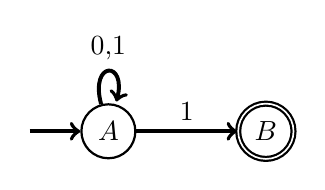
\begin{tikzpicture}[baseline={(s0.base)}]
% \draw[help lines] (0,0) grid (7,2);
\node (s0) [circle,draw=black,thick] at (0,0) {$A$};
\node (s1) [circle,draw=black,thick,double] at (2,0) {$B$};
%
\path[->,line width=0.5mm](-1,0) edge (s0);
\path[->,line width=0.5mm](s0) edge [loop above] node[above] {\Sterm{0},\Sterm{1}} (s0);
\path[->,line width=0.5mm](s0) edge node[above] {\Sterm{1}} (s1);
\end{tikzpicture}\hfill
% 
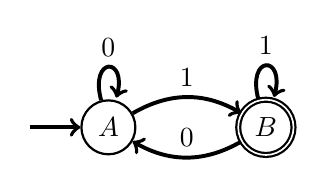
\begin{tikzpicture}[baseline={(s0.base)}]
% \draw[help lines] (0,0) grid (7,2);
\node (s0) [circle,draw=black,thick] at (0,0) {$A$};
\node (s1) [circle,draw=black,thick,double] at (2,0) {$B$};
%
\path[->,line width=0.5mm](-1,0) edge (s0);
\path[->,line width=0.5mm](s0) edge [loop above] node[above] {\Sterm{0}} (s0);
\path[->,line width=0.5mm, bend left](s0) edge node[above] {\Sterm{1}} (s1);
\path[->,line width=0.5mm, bend left](s1) edge node[above] {\Sterm{0}} (s0);
\path[->,line width=0.5mm](s1) edge [loop above] node[above] {\Sterm{1}} (s1);
\end{tikzpicture}}

\begin{itemize}
\item NFA-Minimierung ist algorithmisch aufwändiger
\item \ldots{} und liefert kein eindeutiges Ergebnis,
\item \ldots{} ist aber durchaus praktisch machbar
\end{itemize}
% $\leadsto$ Wir determinisieren Automaten, um sie zu minimieren

\end{frame}

\begin{frame}\frametitle{Sind NFAs wirklich kompakter?}

Beispiel aus Vorlesung 4:
$\Slang{L}_n= \{\Sterm{0},\Sterm{1}\}^* \Sterm{1} \{\Sterm{0},\Sterm{1}\}^{n-1}$
("`Wörter mit \Sterm{1} an $n$-letzter Stelle"')
\bigskip

Wir haben gesehen, dass es dafür NFAs der Größe $n+1$ gibt
\bigskip

DFAs benötigen dagegen mindestens $2^n$ Zustände\pause
\bigskip

\emph{Beweis:} mit Hilfe von Myhill/Nerode:
\begin{itemize}
\item Die Kongruenzklassen haben die Form $[w]_\simeq$ mit $w\in\{\Sterm{0},\Sterm{1}\}^n$
\item Jede dieser Klassen ist unterschiedlich, z.B. für $n=3$:\\
wenn $v\in[\Sterm{011}]$ dann $v\epsilon\notin\Slang{L}_3$, $v\Sterm{0}\in\Slang{L}_3$ und $v\Sterm{00}\in\Slang{L}_3$\\
wenn $v\in[\Sterm{101}]$ dann $v\epsilon\in\Slang{L}_3$, $v\Sterm{0}\notin\Slang{L}_3$ und $v\Sterm{00}\in\Slang{L}_3$\\
\ldots
\item Es gibt also mindestens $2^n$ Kongruenzklassen\\(=Zustände im Minimal-DFA)
\end{itemize}

\end{frame}

\sectionSlide{Ausblick: Nichtreguläre Sprachen}

\begin{frame}\frametitle{Nichtreguläre Sprachen}

Sind alle Sprachen regulär?\\\pause
\redalert{Sicher nicht} (dazu gibt es zu viele Sprachen)\pause
\bigskip

Sind alle Typ-0-Sprachen regulär?\\\pause
\redalert{Nein,} auch das gilt nicht
\bigskip

\alert{Wie aber zeigt man das?}
\begin{itemize}
\item Behauptung "`Sprache $\Slang{L}$ ist regulär!"' $\leadsto$ es genügt, \alert{einen} Automaten, regulären Ausdruck oder eine Typ-3-Grammatik für $\Slang{L}$ anzugeben
\item Behauptung "`Sprache $\Slang{L}$ ist nicht regulär!"' $\leadsto$ man müsste zeigen, dass es \alert{keinen} Automaten, \alert{keinen} regulären Ausdruck bzw. \alert{keine} Typ-3-Grammatik für $\Slang{L}$ gibt
\end{itemize}

\end{frame}

% \begin{frame}\frametitle{Nichtregularität mit Myhill \& Nerode}
% 
% Myhill \& Nerode liefern uns ein besseres Kriterium:
% 
% \theobox{Satz (Myhill \& Nerode): Eine Sprache $\Slang{L}$ ist genau dann regulär, wenn $\simeq_{\Slang{L}}$ endlich viele Äquivalenzklassen hat.}\medskip
% 
% Daraus folgt:
% 
% \theobox{Satz: Wenn $\simeq_{\Slang{L}}$ unendlich viele Äquivalenzklassen, dann ist $\Slang{L}$ nicht regulär.}%
% \medskip\pause
% 
% \examplebox{Beispiel: Wir haben gesehen, dass die Sprache $\{\Sterm{a}^n\Sterm{b}^n\mid n\geq 0\}$
% unendlich viele Äquivalenzklassen erzeugt. Diese Sprache ist demnach nicht regulär.}
% 
% \end{frame}
% 
% \begin{frame}\frametitle{$\Sterm{a}^n\Sterm{b}^n$}
% 
% Die Sprache $\Sterm{a}^n\Sterm{b}^n$ gilt als Musterbeispiel nichtregulärer Sprachen
% \bigskip
% 
% \anybox{purple}{Intuition: "`Reguläre Sprachen können nicht zählen."'}%
% \bigskip
% 
% Ein Automat, der diese Sprache erkennen wollte, müsste die genaue Zahl der schon gelesenen $\Sterm{a}$s speichern
% \medskip
% 
% $\leadsto$ beliebig viel Speicher nötig
% \bigskip
% 
% Viele Sprachdefinitionen mit Bezug zu konkreten Zahlen verhalten sich ähnlich
% 
% \end{frame}
% 
% \begin{frame}[t]\frametitle{Nichtregularität mit Abschlusseigenschaften}
% 
% Wir haben bereits gezeigt:
% 
% \theobox{Satz: Wenn $\Slang{L}_1$ und $\Slang{L}_2$ regulär sind, dann auch $\Slang{L}_1\cap \Slang{L}_2$,
% $\Slang{L}_1\cup \Slang{L}_2$, $\Slang{L}_1^*$ und $\overline{\Slang{L}}_1$.}\medskip
% 
% Auch hier liefert die Umkehrung gute Kriterien, z.B.
% \theobox{Satz: Wenn $\Slang{L}_1$ regulär und $\Slang{L}_1\cap \Slang{L}_2$ nicht regulär ist, dann ist
% $\Slang{L}_2$ ebenfalls nicht regulär.}\medskip
% 
% \examplebox{Beispiel: Wir betrachten über dem Alphabet $\{\Sterm{a},\Sterm{b}\}$ die Sprache $\Slang{L}=\{w\mid w\text{ enthält ebenso viele $\Sterm{a}$ wie $\Sterm{b}$}\}$.
% \medskip
% 
% \only<2->{Dann gilt $\Slang{L}\cap \{\Sterm{a}\}^*\{\Sterm{b}\}^* = \{\Sterm{a}^n\Sterm{b}^n\mid n\geq 0\}$.
% \medskip
% 
% Weil $\{\Sterm{a}\}^*\{\Sterm{b}\}^*$ regulär ist und $\{\Sterm{a}^n\Sterm{b}^n\mid n\geq 0\}$ nicht kann
% $\Slang{L}$ ebenfalls nicht regulär sein.}
% }
% 
% \end{frame}
% 
% % \begin{frame}[t]\frametitle{Nichtregularität mit Abschlusseigenschaften (2)}
% % 
% % Noch ein Beispiel: Komplement der gerade gezeigten Sprache
% % 
% % \end{frame}
% 
% \newcommand{\colstackrel}[3]{\,{\stackrel{\textcolor{#3}{#1}}{\textcolor{#3}{#2}}}\,}
% \newcommand{\gstackrel}[2]{\colstackrel{#1}{#2}{darkgreen}}
% \newcommand{\bstackrel}[2]{\colstackrel{#1}{#2}{darkblue}}
% \newcommand{\rstackrel}[2]{\colstackrel{#1}{#2}{darkred}}
% 
% \begin{frame}\frametitle{Nichtregularität durch Pumpen}
% 
% Ein weiteres klassisches Kriterium für Nichtregularität ist, dass die Wörter regulärer Sprachen
% beliebig "`aufgepumpt"' werden können:
% 
% \theobox{Satz (Pumping Lemma):
% Für jede reguläre Sprache $\Slang{L}$\\
% gibt es eine Zahl $n\geq 0$, so dass gilt:\\
% ~~für jedes Wort $z\in\Slang{L}$ mit $|z|\geq n$\\
% ~~gibt es eine Zerlegung $z=uvw$ mit $|v|\geq 1$ und $|uv|\leq n$, so dass:\\
% ~~~~für jede Zahl $k\geq 0$ gilt: $u v^k w\in\Slang{L}$
% }
% 
% \pause
% \emph{Beweis:} Sei $\Smach{M}$ ein DFA für $\Slang{L}$ mit $|Q|$ Zuständen.
% Wir wählen $n=|Q|+1$. Ein akzeptierender Lauf für ein beliebiges Wort $z$ mit $|z|=\ell\geq n$
% muss in den ersten $n$ Schritten einen Zustand $p$ zweimal besuchen (sagen wir: nach $i$ und $j$ Schritten),
% hat also die Form:
% % Es gibt also Zahlen mit $0\leq i<j\leq n$ für die der Lauf folgende Form hat:
% % Der Lauf hat also folgende Form:
% %
% \[ q_0 \gstackrel{z_1}{\to}q_1\gstackrel{z_2}{\to}\!\ldots\!\gstackrel{z_{i-1}}{\to}q_{i-1}\gstackrel{z_i}{\to} p\bstackrel{z_{i+1}}{\to} q_{i+1}\bstackrel{z_{i+2}}{\to}\!\ldots\!\bstackrel{z_{j-1}}{\to}q_{j-1}\bstackrel{z_j}{\to} p \rstackrel{z_{j+1}}{\to}q_{j+1}\rstackrel{z_{j+2}}{\to}\!\ldots\!\rstackrel{z_\ell}{\to}q_\ell\]
% %
% Die gesuchte Zerlegung ist $u=\textcolor{darkgreen}{z_1\cdots z_i}$, $v=\textcolor{darkblue}{z_{i+1}\cdots z_{j}}$, $w=\textcolor{darkred}{z_{j+1}\cdots z_\ell}$.
% Der Lauf $(q_0\ldots q_{i-1} p) (q_{i+1}\ldots q_{j-1}p)^k (q_{j+1}\ldots q_\ell)$ akzeptiert $uv^k w$.
% % 
% % Akzeptierende Läufe für $uv^k w$.
% % 
% % 
% % Es gibt also einen
% % Zyklus $q\stackrel{v}{\to}q$. Die Behauptung folgt, da man diesen Zyklus beliebig oft durchlaufen kann.
% \qed
% 
% \end{frame}
% 
% \begin{frame}\frametitle{Beispiel}
% 
% \examplebox{%
% Beispiel: Die Sprache von $\Sterm{b}^*(\Sterm{a}\Sterm{b}^*\Sterm{a}\Sterm{b}^*)^*$ (Wörter mit gerader Anzahl $\Sterm{a}s$).
% Der Parameter $n$ aus dem Pumping-Lemma kann $2$ sein:
% \begin{itemize}
% \item Wenn $z$ die Form $\Sterm{b}y$ hat, wähle $u=\epsilon$, $v=\Sterm{b}$ und $w=y$
% \item Wenn $z$ die Form $\Sterm{ab}y$ hat, wähle $u=\Sterm{a}$, $v=\Sterm{b}$ und $w=y$
% \item Wenn $z$ die Form $\Sterm{aa}y$ hat, wähle $u=\epsilon$, $v=\Sterm{aa}$ und $w=y$
% \end{itemize}
% }\medskip\pause
% 
% \examplebox{Beispiel: Für endliche Sprachen ist die Eigenschaft trivial. Man wählt $n$ einfach so groß, dass
% es keine Wörter $z$ mit $|z|\geq n$ gibt, für welche weitere Eigenschaften gefordert werden.}
% 
% \end{frame}
% 
% \begin{frame}[t]\frametitle{Pumpen für Nichtregularität}
% 
% Die Pump-Eigenschaft ist für Regularität \alert{notwendig}, aber \alert{nicht hinreichend}: man kann auch manche nichtreguläre Sprachen pumpen.
% \medskip
% 
% Daher eignet sich das Pumping-Lemma eher zum Beweis der Nichtregularität
% \medskip\pause
% 
% \examplebox{Beispiel: Sei $\Slang{L}=\{\Sterm{a}^k\mid k\text{ ist Primzahl}\}$.
% \only<3->{\medskip
% 
% Angenommen es gäbe einen Wert $n$ für den diese Sprache aufgepumpt werden kann.
% Es gibt eine Primzahl $\ell>n+2$.
% Laut Pump-Eigenschaft finden wir eine Zerlegung von $\Sterm{a}^\ell=uvw$
% für die insbesondere gilt $uv^{|uw|}w\in\Slang{L}$.
% Aber $uv^{|uw|}w=\Sterm{a}^{(k+1)|uw|}\notin\Slang{L}$. Widerspruch.\medskip
% 
% $\Slang{L}$ ist daher nicht regulär.}
% }
% 
% \end{frame}
% 
% 
% \begin{frame}\frametitle{Ist das Pumping-Lemma sinnvoll?}
% 
% % Diskussion:
% \begin{itemize}
% \item \emph{Kontra:} Myhill-Nerode liefert ein notwendiges \redalert{und} hinreichendes Kriterium für Regularität\\
% $\leadsto$ immer anwendbar, um (Nicht)Regularität zu zeigen
% \item \emph{Pro:} Pumping funktioniert in den allermeisten praktischen Fällen auch\\
% (notfalls kann man Abschlusseigenschaften zu Hilfe nehmen)
% \item \emph{Pro:} Manchmal ist der Beweis mit Pumping einfacher
% \item \emph{Kontra:} Das formale Pumping Lemma ist relativ kompliziert
% \item \emph{Pro:} Die Punmping-Idee ist intuitiv und wir werden sie später noch einmal bei kontextfreien Sprachen nutzen
% \end{itemize}
% 
% \end{frame}

\begin{frame}\frametitle{Zusammenfassung und Ausblick}

Der \redalert{Satz von Myhill und Nerode} charakterisiert reguläre Sprachen und liefert einen direkt konstruierten DFA für eine Sprache
\bigskip

Der \redalert{reduzierte DFA} ist minimal und eindeutig
\bigskip

NFAs können viel kleiner sein als minimale DFAs, aber ihre Minimierung ist viel komplizierter

% \redalert{Nichtregularität} von Sprachen kann man mit Myhill-Nerode, Abschlusseigenschaften und Pumping nachweisen

\anybox{yellow}{
Offene Fragen:
\begin{itemize}
\item Wie findet man nichtreguläre Sprachen?
\item Welche weiteren Berechnungsaufgaben gibt es im Zusammenhang mit regulären Sprachen?
% \item Wie aufwändig sind die verschiedenen Konstruktionen und Berechnungen?
\item Und was ist mit kontextfreien Sprachen?
\end{itemize}
}

\end{frame}


\end{document}
